\subsection{Tipo de entidad Calificación Alumno Asignatura CA}

   \begin{description}

   \item[Definición] Se refiere al objeto del mundo real: \emph{``Calificación
   obtenida por un alumno en una determinada asignatura durante un curso
   académico''}.

   \item[Características] La entidad presenta las siguientes características:
      \begin{itemize}
         \item \textbf{Nombre:} Calificación Alumno Asignatura CA.
         \item \textbf{Tipo:} Débil por identificación con respecto a las
         entidades Alumno Curso Académico y Asignatura Curso Académico.
         \item \textbf{Número de atributos:} 3 propio y 5 heredados.
         \item \textbf{Atributo/s identificador/es principal/es:} dni\_pasaporte
         junto con curso\_académico, id\_centro, id\_titulación, id\_asignatura
         y convocatoria.
         \item \textbf{Atributo/s identificador/es alternativo/s:} -
         \item \textbf{Atributo/s heredado/s:} dni\_pasaporte y curso\_académico del tipo de entidad Alumno Curso Académico, además de id\_centro, id\_titulación
         e id\_asignatura del tipo de entidad Asignatura Curso Académico.
      \end{itemize}

   \item[Diagrama] La figura \ref{diagramaCalAlACA} muestra el diagrama de la entidad.
   \item \begin{figure}[!ht]
            \begin{center}
            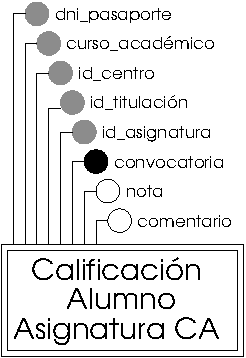
\includegraphics[]{07.Modelo_Entidad-Interrelacion/7.2.Analisis_Entidades/diagramas/cal_al_aca.pdf}
            \caption{Diagrama de la entidad Calificación Alumno Asignatura CA.}
            \label{diagramaCalAlACA}
            \end{center}
         \end{figure}

   \item[Descripción de los atributos propios] La entidad presenta los
   siguientes atributos propios:

   \begin{itemize}
    \item \textbf{convocatoria}
    \begin{itemize}
      \item \textbf{Definición:} Establece la convocatoria en la que el
      alumno se presenta a la asignatura.
      \item \textbf{Dominio:} Conjunto de caracteres alfanuméricos.
      \item \textbf{Carácter:} Obligatorio.
      \item \textbf{Ejemplo práctico:} febrero.
      \item \textbf{Información adicional:} Es clave primaria de la
      entidad. El dato lo introduce el usuario alumno al actualizar
      su información personal, o bien el usuario asesor si
      comprueba que la información no es correcta.
    \end{itemize}
    \item \textbf{nota}
    \begin{itemize}
      \item \textbf{Definición:} Establece la calificación obtenida por un
      alumno en una asignatura durante un curso académico.
      \item \textbf{Dominio:} Conjunto de reales positivos.
      \item \textbf{Carácter:} Opcional.
      \item \textbf{Ejemplo práctico:} 8,4.
      \item \textbf{Información adicional:} El dato lo introduce el
      usuario alumno al actualizar su información personal , o
      bien el usuario asesor si comprueba que la información no es
      correcta.
    \end{itemize}
    \item \textbf{comentario}
    \begin{itemize}
      \item \textbf{Definición:} Información extra que pueda ser
      interesante conocer.
      \item \textbf{Dominio:} Conjunto de caracteres alfanuméricos.
      \item \textbf{Carácter:} Opcional.
      \item \textbf{Ejemplo práctico:} Prácticas superadas.
      \item \textbf{Información adicional:} El dato lo introduce el
      usuario alumno al actualizar su información personal , o
      bien el usuario asesor si comprueba que la información no es
      correcta.
    \end{itemize}
   \end{itemize}

   \item[Ejemplo práctico]

   \item \begin{center}
            \begin{tabular}{ | l | l | }
            \hline
            \multicolumn{2}{ | c | }{\textbf{Tipo de entidad Calificación Alumno Asignatura CA}} \\
            \hline
            dni\_pasaporte & 01234567A \\
            \hline
            curso\_académico & 2008 \\
            \hline
            id\_centro & 15 \\
            \hline
            id\_titulación & 3\\
            \hline
            id\_asignatura & 17\\
            \hline
            convocatoria & febrero \\
            \hline
            nota & 8,4 \\
            \hline
            comentario & Prácticas superadas \\
            \hline
            \end{tabular}
         \end{center}
   \end{description}
